\documentclass[conference]{IEEEtran}
\IEEEoverridecommandlockouts
% The preceding line is only needed to identify funding in the first footnote. If that is unneeded, please comment it out.
\usepackage{cite}
\usepackage{amsmath,amssymb,amsfonts}
\usepackage{algorithmic}
\usepackage{graphicx}
\usepackage{textcomp}
\usepackage{xcolor}
\usepackage{caption}


\def\BibTeX{{\rm B\kern-.05em{\sc i\kern-.025em b}\kern-.08em
    T\kern-.1667em\lower.7ex\hbox{E}\kern-.125emX}}
\begin{document}

\pagestyle{plain}

\title{DAL 2023 - Assignment 1\\
{\footnotesize }

}

\author{\IEEEauthorblockN{Pranoy K P}
\IEEEauthorblockA{\textit{Engineering Design} \\
\textit{Indian Institute of Technology, Madras}\\
\textit{Chennai, Tamil Nadu} \\
\textit{ed20b045@smail.iitm.ac.in}
}
}

\maketitle

\begin{abstract}
This study uses the provided dataset to explore the correlation of socioeconomic status with cancer incidence and mortality rates in the United States. The study’s findings highlight the need for targeted interventions and policy changes to address these health disparities. The visualisations created by the analysis can be used to advocate for policy change and fundraising for improved health equity. This paper aims to learn about the mathematical principles of linear regression and apply them to solve a real-world problem.
\end{abstract}

\section{INTRODUCTION}
This study uses a cancer incidence and mortality rates dataset in the United States to explore their correlation with socioeconomic status. The study’s findings highlight the need for targeted interventions and policy changes to address these health disparities. These interventions and policy changes could include providing more affordable health insurance, increasing access to cancer screening and treatment, and educating people about cancer prevention. The visualisations created by the dataset analysis can be used to advocate for policy change and fundraising for improved health equity. These visualisations can help communicate the study’s findings to policymakers and the public and can help raise awareness of the issue of cancer disparities.

The paper aims to learn about the mathematical principles of linear regression and apply them to solve real-world problems. Linear regression is the statistical approach to finding a linear relationship between variables. In this case, the variables we are trying to predict are cancer incidence and mortality rates. We use the mathematical principles of linear regression to develop a model that can indicate cancer incidence or mortality rates based on socioeconomic status. We then use this model to plot the relation between different groups’ poverty, median income, health insurance, cancer incidence, and mortality rates.

The central issue is whether a correlation exists between socioeconomic status, income, and the likelihood of cancer diagnosis and mortality. Low-income communities often face barriers to accessing quality healthcare, preventive measures, and early detection. Understanding these connections can aid in identifying areas where interventions are needed most urgently. By addressing this problem, we aim to provide empirical evidence that can guide our nonprofit client’s efforts in advocating for improved healthcare policies and securing resources for low-income populations affected by cancer.

This paper presents a comprehensive analysis combining statistical analysis with a deep understanding of social healthcare disparities. We commence by exploring the dataset and its relevance to our research objectives. Subsequently, we delve into the methodology, applying linear regression to investigate the relationships between income levels and cancer outcomes. The results shed light on the disparities low-income individuals face regarding cancer diagnosis and mortality. 

\vspace{1mm} %vertical space

\section{LINEAR REGRESSION}

\subsection{Definition}
Linear regression is a supervised machine learning algorithm that computes the linear relationship between a dependent variable and one or more independent features. The algorithm aims to find the best linear equation that can predict the value of the dependent variable based on the independent variables. The equation provides a straight line that represents the relationship between the dependent and independent variables. The slope of the line indicates how much the dependent variable changes for a unit change in the independent variable(s).

\begin{equation}
y(x) = w^Tx + b
\end{equation}

\begin{figure}[htbp]
\centerline{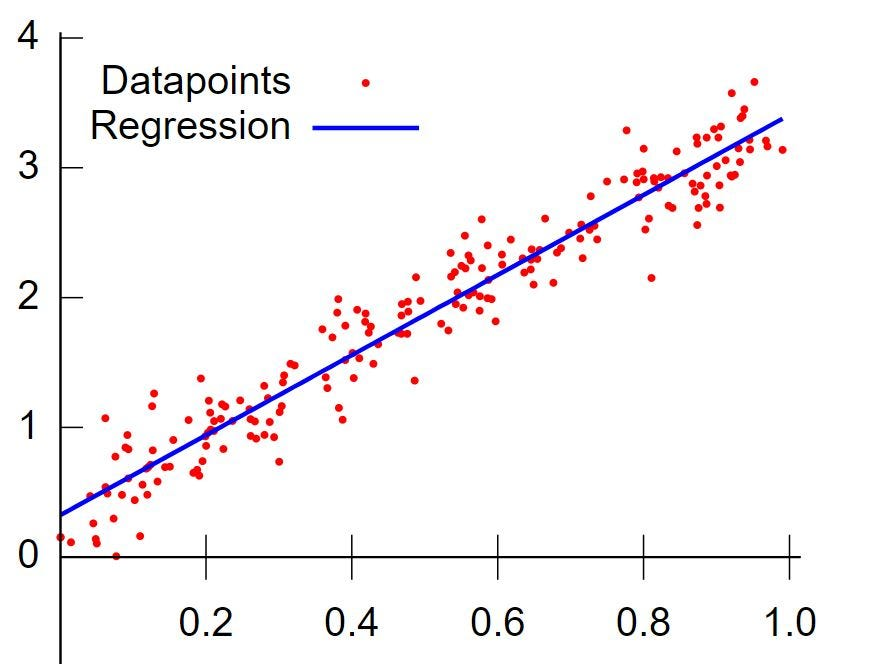
\includegraphics[scale = 0.25]{linear regression.jpg}}
\caption{Linear Regression}
\label{fig}
\end{figure}

\subsection{Cost Function}
The cost function measures the performance of a machine learning model for a data set. The cost function quantifies the error between predicted and expected values and presents that error as a single real number. In the linear regression model, it is the Root Mean Squared Error between the predicted value and true value.
\begin{equation}
J(w,b) = \frac{1}{2m} \sum_{i=1}^{m} (y^{(i)} - (w^T x^{(i)} + b))^2
\end{equation}

\subsection{Gradient Descent}
Gradient Descent is one of the most commonly used optimization algorithms to train machine learning models by minimizing errors between actual and expected results. The gradient points in the direction of the steepest increase in the function, and moving in the opposite direction leads to the most significant reduction in the cost. During each iteration, we reduce the cost moving along this direction, and the size of each step is determined by the hyperparameter known as the learning rate \(\alpha\). This iterative process continues until a stopping criterion is met.

The choice of the learning rate is crucial. If it's too small, it would require excessive iterations to converge. Conversely, if it's too large, the optimization process can become unstable, causing the output to oscillate and potentially diverge from the optimal solution. Therefore, finding an appropriate learning rate is crucial to gradient descent optimization.

A few types of gradient descent are Batch Gradient Descent, Stochastic Gradient Descent, Mini-Batch Gradient Descent, Momentum Gradient Descent, Nesterov Accelerated Gradient, Adagrad, RMSprop (Root Mean Square Propagation) and Adam (Adaptive Moment Estimation), 

\vspace{1mm} %vertical space

\section{THE PROBLEM}
In this section, we will conduct a case study on whether socio-economic factors such as income, poverty, and health insurance subscriptions are related to cancer incidence and mortality. Linear Regression technique is used to understand our plots better and strengthen our claim.

\subsection{Exploratory Data Analysis}
We know that linear regression works based on the assumption that the conditional distribution of the target variable is normal. Below is the distribution of the Mortality Rate and Incidence Rate.

\begin{figure}[htbp]
\centerline{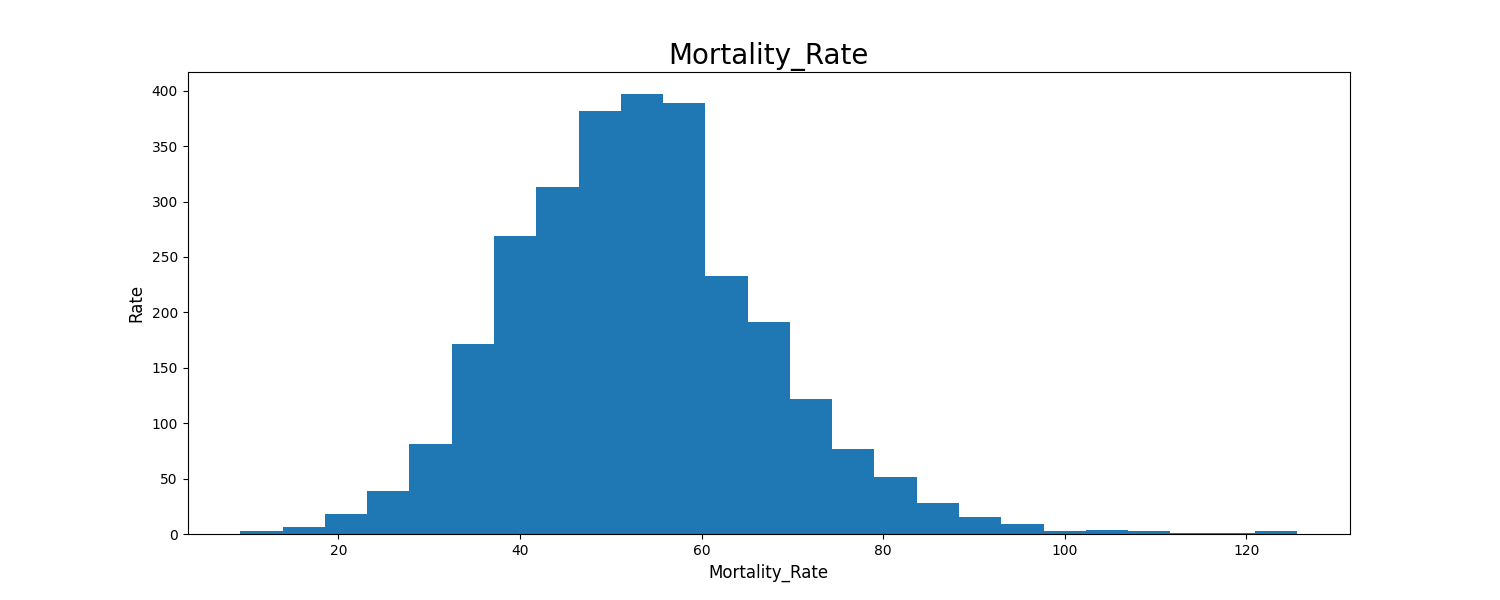
\includegraphics[scale = 0.27]{Mortality_Rate.png}}
\caption{Mortality Rate Distribution}
\label{fig}
\end{figure}

\begin{figure}[htbp]
\centerline{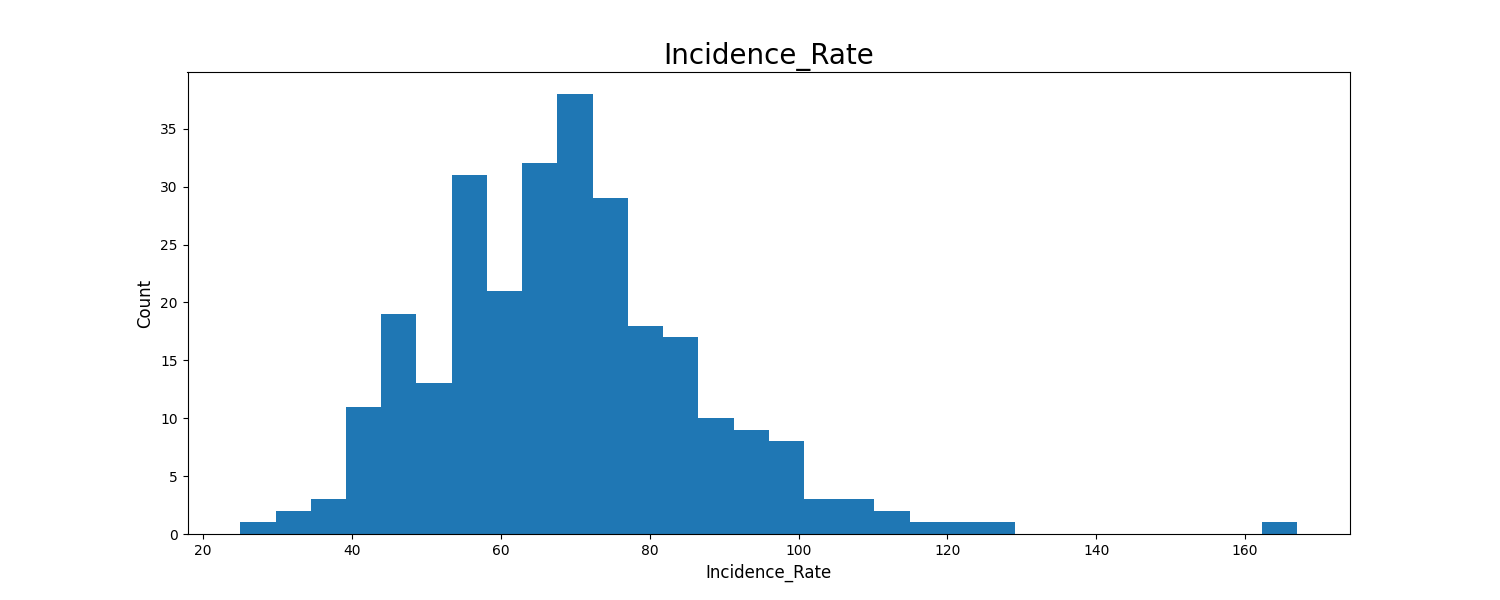
\includegraphics[scale = 0.24]{Incidence_Rate.png}}
\caption{Incidence Rate Distribution}
\label{fig}
\end{figure}
From these figures, we can see that our target variables follow the normal distribution. Hence, applying a linear regression model could be a good choice.

\subsection{Data Cleaning}
We follow up by cleaning our data. Taking a quick look at all column entries, we can easily make out that several features, for example, the data on median income of different ethnicities, have a lot of missing or non-numeric values. We must find the essential features from the cleaned data version to train our model more accurately. The first three columns, namely 'Unnamed', 'State', and 'AreaName', are removed since they don't provide valuable information to our analysis. Similarly, we avoid the 'FIPS', 'fips\_x', and 'fips\_y' values as they are essentially unique positional identifiers for the different counties.

\subsection{Modelling}
After cleaning the data and narrowing down the independent variables, we attempt to fit the linear model over the training data. Firstly, we seek insights by visualising socioeconomic factors versus incidence and mortality rates separately. The following socio-economic factors have been considered for the analysis. 

\subsubsection{Poverty}
In the following plots, we visualize whether there is any correlation between poverty and incidence and mortality rates. The absolute number of people living in poverty may not be helpful. Plots are constructed between the poverty percentage and the target variables, where poverty percentage is defined as the count of people living in poverty in an area by the estimated population (in per cent) of that area.

\begin{figure}[htbp]
\centerline{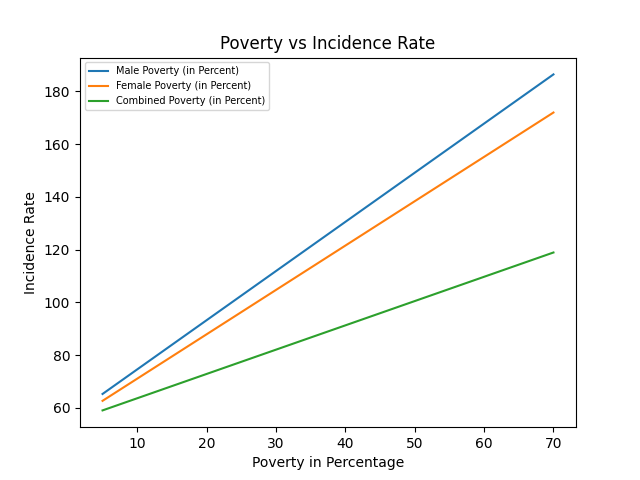
\includegraphics[scale = 0.58]{Poverty vs Incidence Rate.png}}
\caption{Poverty vs. Incidence Rate}
\label{fig}
\end{figure}

Fig. 4 strengthens the evidence that the incidence rate increases as the poverty percentage increases. Access to good healthcare and proper nutrition is difficult for impoverished people. Male and female poverty show similar trends, implying that gender does not impact much on the incidence rate.

\begin{figure}[htbp]
\centerline{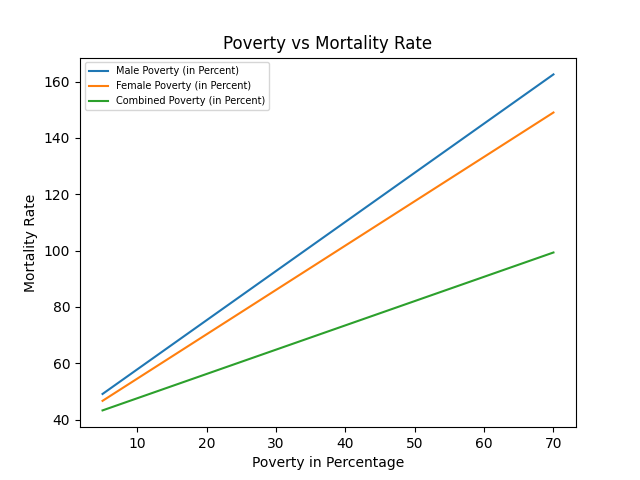
\includegraphics[scale = 0.58]{Poverty vs Mortality Rate.png}}
\caption{Poverty vs. Mortality Rate}
\label{fig}
\end{figure}

Similar trends are observed across Poverty versus Mortality Rate. Similar patterns emerge, suggesting that impoverished impoverished individuals are more vulnerable to cancer and related diseases than their more economically advantaged counterparts.

\subsubsection{Income}
This section will analyse how income impacts cancer incidences and mortality rates. We attempt to do this using graphs of the Median Income vs. Incidence and Mortality Rates for different ethnicities.

\begin{figure}[htbp]
\centerline{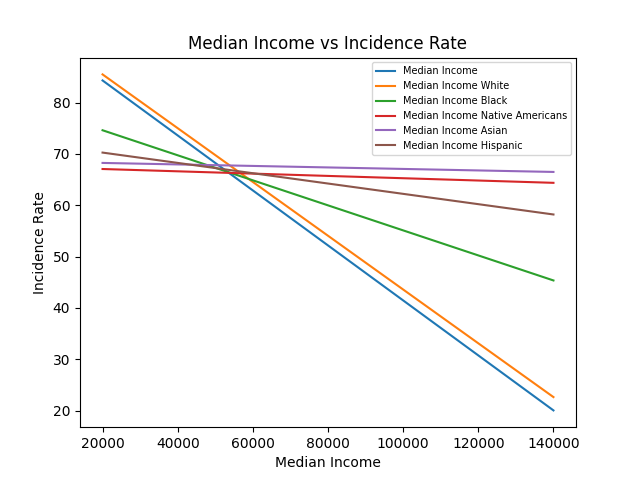
\includegraphics[scale = 0.58]{Median Income vs Incidence Rate.png}}
\caption{Median Income vs. Incidence Rate}
\label{fig}
\end{figure}

From Fig. 6, it is evident that income does play a role. People with lower incomes have difficulty managing healthcare expenses and obtaining nutritious food. This could also be attributed to income being closely related to poverty. Hence, such a trend could have been observed.

\begin{figure}[htbp]
\centerline{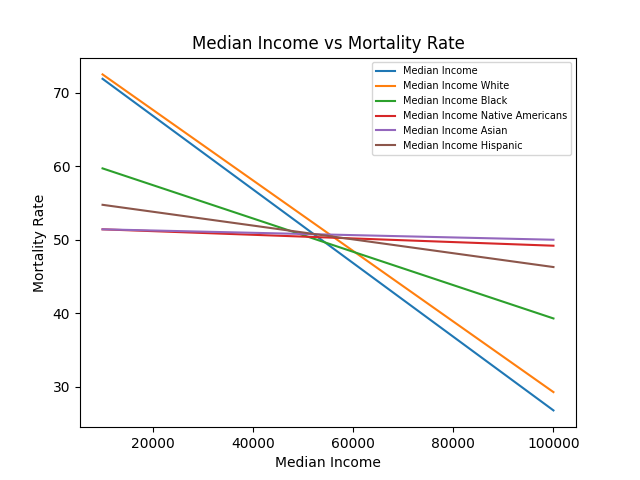
\includegraphics[scale = 0.58]{Median Income vs Mortality Rate.png}}
\caption{Median Income vs. Mortality Rate}
\label{fig}
\end{figure}

Fig. 7 shows that the mortality rate of lower-income people is high and decreases steeply as income increases. This substantiates that people with lower incomes are more susceptible to death due to cancer.

One thing to be noted is that while the conclusion is undeniable from the graph for people of white ethnicity, it is not so straightforward for other groups. This may be due to discrepancies in data collection from people of other races. Due to the missing data for different ethnicities, the trend has not been captured clearly.

\subsubsection{Health Insurance}
This section explores whether individuals covered by health insurance possess a distinct advantage and are comparatively less susceptible to cancer incidence and mortality. Our analysis will encompass various demographic segments, including gender-specific differences and the general population, as we unravel the correlation between the variables.

Once again, the absolute count of people with Health Insurance may not be helpful. So, plots are constructed for the percentage of people with health insurance versus the target variables, Incidences and Mortality Rates. Percentages are number of people with Health Insurance per estimated population of an area.

\begin{figure}[htbp]
\centerline{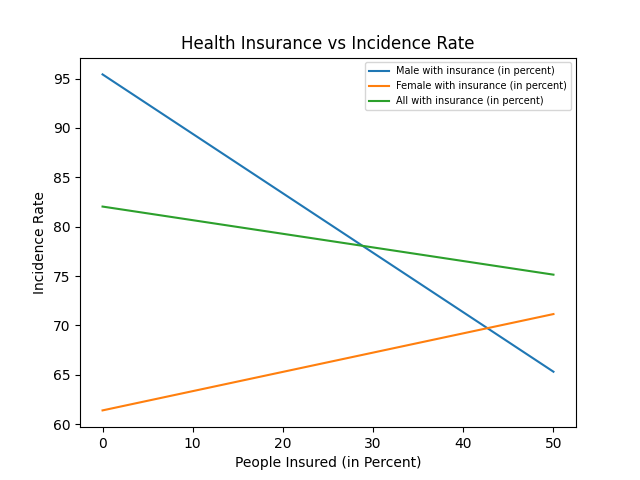
\includegraphics[scale = 0.58]{Health Insurance vs Incidence Rate.png}}
\caption{Health Insurance vs. Incidence Rate}
\label{fig}
\end{figure}

As evident from Fig. 8, Cancer incidence is slightly lower in areas with high insurance percentages than in areas with low insurance percentages. This is because insurance is usually obtained after a medical diagnosis and does not significantly impact the likelihood of developing cancer. The slight decrease in cancer incidence rates in areas with high insurance percentages could be because higher-income people are more likely to have health insurance. However, this does not necessarily mean that health insurance effectively prevents cancer, as people with lower incomes may also seek health insurance in case of a cancer diagnosis. The effect is clearly on display for men. Also, the cancer incidence rates for women with health insurance are slightly higher or remain the same as those without health insurance. Therefore, more research is needed to determine the true impact of health insurance on cancer incidence rates.

\begin{figure}[htbp]
\centerline{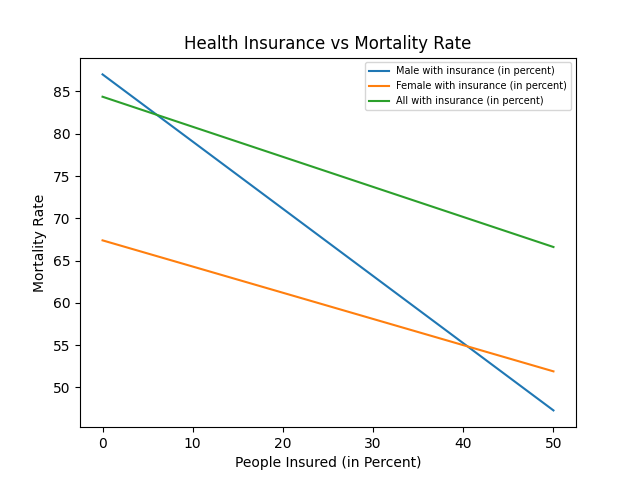
\includegraphics[scale = 0.58]{Health Insurance vs Mortality Rate.png}}
\caption{Health Insurance vs. Mortality Rate}
\label{fig}
\end{figure}

From Fig. 9, the mortality rate decreases as the percentage of people with health insurance increases. This is because people with health insurance are more likely to receive timely and quality medical care, which can improve their chances of survival. This study's findings differ from previous studies on the relationship between health insurance and cancer incidence. This might be because the probability of getting diagnosed with cancer is not significantly affected by health insurance. Still, the chances of survival can be improved by having health insurance.

\subsubsection{Statistical Analysis}
In this section, we employ statistical methodologies to interpret the data. Statistical analysis helps us quantify relationships between the variables and their chance of incidence. This allows us to derive insights from the dataset provided. The inferences drawn from these tools provide insights into the data that are not visible from the plots to the plain eye.

The p-value is a number calculated from a statistical test that describes how likely you are to have found a particular set of observations if the null hypothesis were true. P-values are used in hypothesis testing to help decide whether to reject the null hypothesis. The smaller the p-value, the more likely you will reject the null hypothesis.

F-statistic, or F-value, is used in regression analysis to identify whether the means between two populations are significantly different. Individual t-tests assume that each variable comes from an independent distribution, which may not always be accurate. In other words, the F-statistic is the ratio of two variances (Variance is nothing but a measure of dispersion; it tells how far the data is dispersed from the mean). F-statistic accounts for corresponding degrees of freedom to estimate the population variance.

R-squared (R²) is a statistical measure in a regression model that determines the proportion of variance in the dependent variable that the independent variable can explain. In other words, r-squared shows how well the data fit the regression model (the goodness of fit). R-squared can take any value between 0 and 1. The closer the R-squared is to 1, the more likely the relationship is statistically linear. 

\begin{table}[h!]
  \begin{center}
    \caption{{Poverty Percentage}}
    \label{tab:table1}
    \begin{tabular}{c|c|c} % <-- Alignments: 1st column left, 2nd middle and 3rd right, with vertical lines in between
      \textbf{Metric} & \textbf{Incidence Rate} & \textbf{Mortality Rate}\\
      \hline
      F statistic & 315.3 & 454.5\\
      P value & 0.000 & 0.001\\
      R squared & 0.107 & 0.147\\
    \end{tabular}
  \end{center}
\end{table}

\begin{table}[h!]
  \begin{center}
    \caption{{Median Income}}
    \label{tab:table1}
    \begin{tabular}{c|c|c} % <-- Alignments: 1st column left, 2nd middle and 3rd right, with vertical lines in between
      \textbf{Metric} & \textbf{Incidence Rate} & \textbf{Mortality Rate}\\
      \hline
      F statistic & 444.8 & 652.2\\
      P value & 0.000 & 0.000\\
      R squared & 0.144 & 0.198\\
    \end{tabular}
  \end{center}
\end{table}

\begin{table}[h!]
  \begin{center}
    \caption{{Health Insurance}}
    \label{tab:table1}
    \begin{tabular}{c|c|c} % <-- Alignments: 1st column left, 2nd middle and 3rd right, with vertical lines in between
      \textbf{Metric} & \textbf{Incidence Rate} & \textbf{Mortality Rate}\\
      \hline
      F statistic & 3.903 & 41.26\\
      P value & 0.048 & 0.000\\
      R squared & 0.001 & 0.015\\
    \end{tabular}
  \end{center}
\end{table}

All models except Health Insurance vs. Incidence Rate have high F-statistic values, implying some relationship between dependent and predictor variables. Though the R-squared value is less, which suggests that the actual relationship could be non-linear, one can see that the p-values of features are less than 0.05, strengthening the conclusions made in the above section. 

For the model between Health Insurance and Incidence Rate, the p-value lies slightly above 0.05, indicating that the linear regression model may not be statistically significant. The F-statistic and the R-squared metrics are among the lowest, meaning that the linear model would be inconclusive. This suggests our claim that Health Insurance doesn’t have a statistical influence on Incidence Rate as Insurance is usually availed after medical treatment and doesn’t influence much on the probability of getting cancer.

\vspace{1mm} %vertical space

\section{CONCLUSIONS}

The study shows that socioeconomic factors such as income, poverty, and access to health insurance can influence cancer incidence and mortality rates. People with higher incomes and lower poverty levels are less likely to develop cancer and more likely to survive if they do develop cancer. This is because they have better access to healthcare, can afford preventive care, and can afford the cost of treatment.

Health insurance is not very effective in preventing cancer, but it can help reduce mortality rates. This is because people with health insurance are more likely to receive timely and quality medical care, which can improve their chances of survival. Targeted programs should be developed to help prevent cancer mortalities in populations with low incomes and high poverty levels. These programs could include incentives for health insurance enrollment, decreased hospital charges, and increased access to preventive care.

Possible research areas could include analyzing the percentage of people with access to sound healthcare systems and why people do not pursue health insurance. This could include factors such as the lack of affordable plans or awareness of health insurance benefits. Another area of interest could be investigating the impact of geographical location on healthcare access, as better quality services and infrastructure are provided in well-off areas, even for economically challenged sections of society.

\begin{thebibliography}{10}
\bibitem{b1}Aurelian Geron, Hands-On Machine Learning with Scikit-Learn, Keras, and TensorFlow: Concepts, Tools and Techniques to Build Intelligent Systems, O'Reilly Media, Inc., pp. 33–143
\bibitem{b2}Bishop Christopher M.. 2006. Pattern Recognition and Machine Learning. Springer.  pp.138-178.
\bibitem{b3}Howlader N, Noone AM, Krapcho M, Miller D, Bishop K, Altekruse SF, Kosary CL, Yu M, Ruhl J, Tatalovich Z, Mariotto A, Lewis DR, Chen HS, Feuer EJ, Cronin KA (eds). SEER Cancer Statistics Review, 1975-2013, National Cancer Institute. Bethesda, MD, https://seer.cancer.gov/archive/csr/1975-2013/, based on November 2015 SEER data submission, posted to the SEER website, April 2016.
\bibitem{b4}Zavala VA, Bracci PM, Carethers JM, Carvajal-Carmona L, Coggins NB, Cruz-Correa MR, Davis M, de Smith AJ, Dutil J, Figueiredo JC, Fox R, Graves KD, Gomez SL, Llera A, Neuhausen SL, Newman L, Nguyen T, Palmer JR, Palmer NR, Pérez-Stable EJ, Piawah S, Rodriquez EJ, Sanabria-Salas MC, Schmit SL, Serrano-Gomez SJ, Stern MC, Weitzel J, Yang JJ, Zabaleta J, Ziv E, Fejerman L. Cancer health disparities in racial/ethnic minorities in the United States. Br J Cancer. 2021 Jan;124(2):315-332. Doi: 10.1038/s41416-020-01038-6. Epub 2020 Sep 9. PMID: 32901135; PMCID: PMC7852513.

\end{thebibliography}

\vspace{12pt}

\end{document}